\chapter{Methodology}
\label{chapter:methodology}

\begin{introduction}
"The things we lose have a way of coming back to us in the end,

if not always in the way we expect"

- J.K. Rowling, Harry Potter and the Order of the Phoenix (2003)
\end{introduction}

As previously mentioned, this research is separated into key stages. This section outlines the beginning of the design of the system's structure by defining its architecture, features, and workflows. To meet the acceptance criteria for this stage and take into account the volume of this research, a strategic framework was selected to guide the architectural design of the proposed solution. By leveraging the principles and steps of \ac{acdm}, this chapter defines the solution's initial requirements, stakeholders, challenges and architecture.

\section{\acl{acdm}} \label{section:acdm}

The \ac{acdm} is a software development methodology, mainly inspired by Quality Attribute Workshop, Architecture Tradeoff Analysis Method and Attribute Driven Design, that emphasises the use of software architecture as a primary driver for the development process \cite{Lattanze2005}. It integrates architectural design into the overall lifecycle of software development, aiming to improve quality, predictability, and efficiency. Below are the key aspects of \ac{acdm} based on the provided paper. \ac{acdm} is structured around the concept that software architecture serves as the backbone of the system, providing a framework for ensuring consistency, scalability, and alignment with business goals. The architecture is not only a technical construct but also a means of communication among stakeholders.

As shown in figure \ref{fig:acdm_workflow}, the \ac{acdm} organises the architectural design process into clearly defined stages that evolve iteratively to ensure a robust, well-aligned system architecture. \ac{acdm} is inherently iterative, with the flexibility to revisit earlier stages based on findings or changing requirements.

\begin{figure}[!htb]
    \caption[\acl{acdm} Workflow]{\ac{acdm} workflow, illustrating the iterative stages, the flow of artifacts, decisions, and refinements through the development process. Adapted from \citeauthoryear{Lattanze2005}.}
    \label{fig:acdm_workflow}
    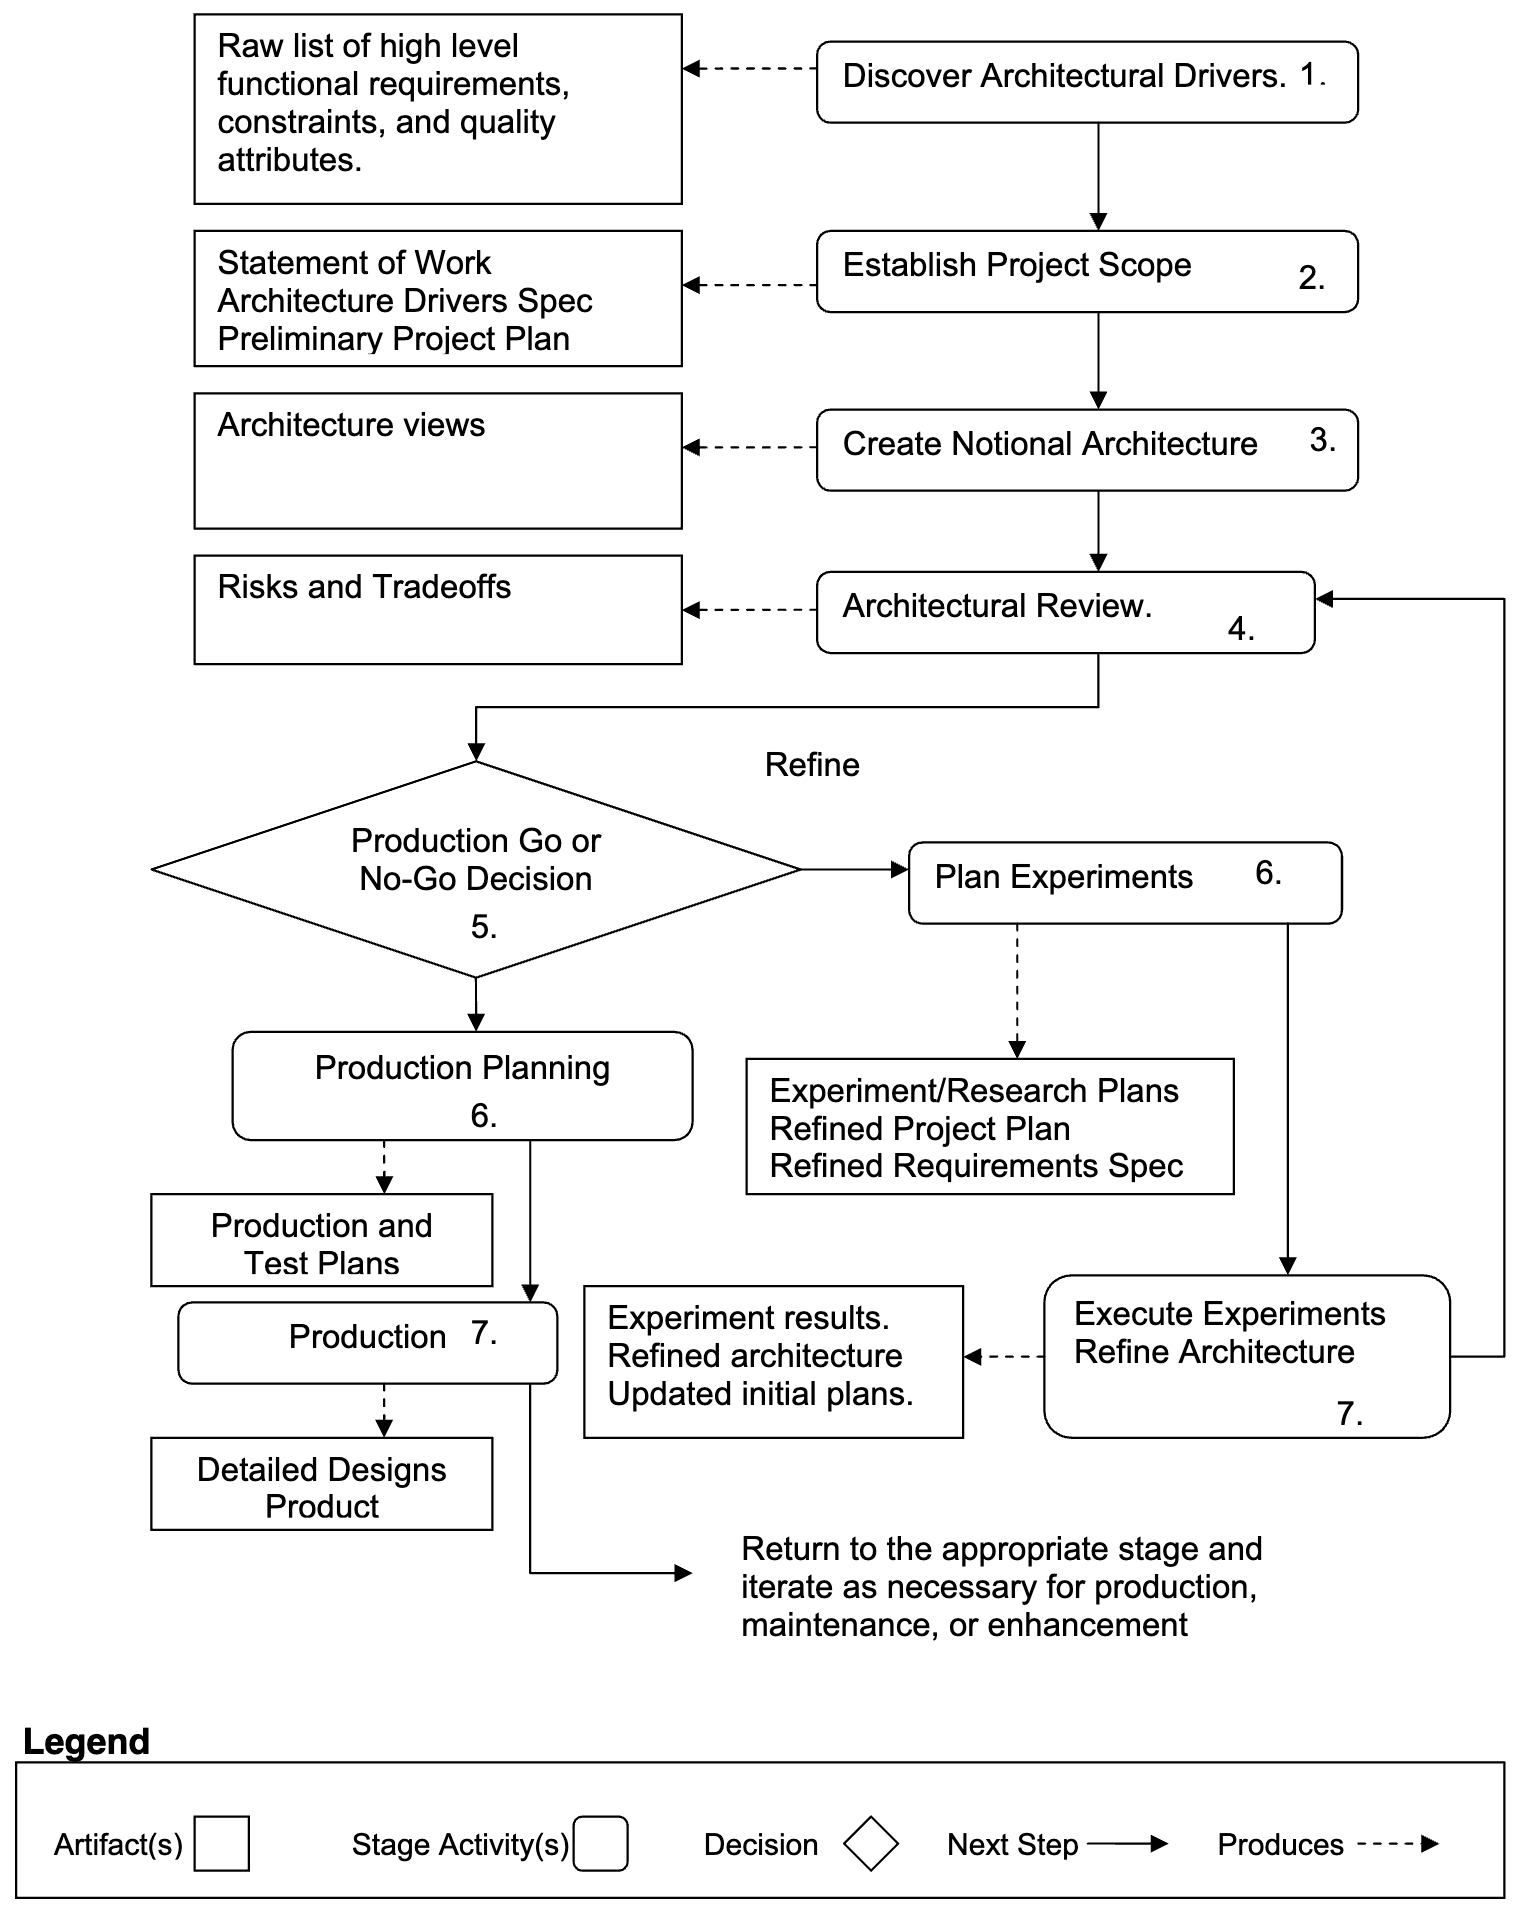
\includegraphics[width=0.6\textwidth]{figs/chapter3/acdm_workflow.png}
    \centering
\end{figure}

According to \citeauthoryear{Lattanze2005}, the process begins with \textbf{Discovering Architectural Drivers}, where critical factors such as functional requirements, quality attributes (e.g., performance, scalability, security), and constraints are identified. These drivers form the foundation for all subsequent design decisions. Following this, the \textbf{Project Scope} is established to define the system's boundaries, objectives, deliverables, and constraints, ensuring all stakeholders have a shared understanding of the project's limits and expectations. Once the drivers and scope are defined, a \textbf{Notional Architecture} is created as a high-level conceptual design. This step involves decomposing the system into components, defining their responsibilities, interactions, and dependencies, and adopting appropriate architectural styles and patterns. The notional architecture serves as a blueprint for early-stage validation. The design is then subjected to an \textbf{Architectural Review}, where it is assessed against the architectural drivers and project scope. Scenario-based evaluations, risk assessments, and stakeholder feedback are key activities during this stage. The outcome is a decision to either proceed to production or refine the architecture further.

If the architecture is deemed insufficient during the review, the process enters a \textbf{Refinement Phase}. This phase begins with \textbf{Experiment Planning}, where targeted experiments are designed to address specific weaknesses or uncertainties, such as performance bottlenecks or scalability challenges. These experiments are executed in the \textbf{Experiment Execution} and \textbf{Architecture Refinement} stage, with findings informing updates to the architecture. Once refined, the updated architecture undergoes another review to ensure it meets the required standards before moving forward.

If the architecture passes the review, the process transitions to the \textbf{Production Phase}, beginning with \textbf{Production Planning}, which involves preparing the system for deployment by developing detailed plans, establishing monitoring mechanisms, and ensuring operational readiness. Finally, the system is deployed during the \textbf{Production} stage, when it becomes operational and accessible to end-users. Post-deployment, the architecture is continuously monitored for performance and feedback, allowing iterative improvements as needed.